\begin{figure}[hbt!]
    \begin{subfigure}[b]{0.5\textwidth}
        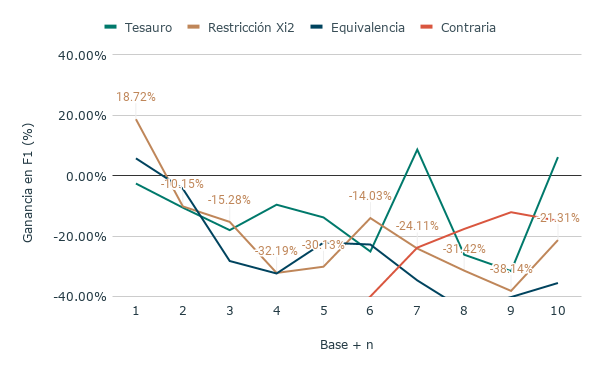
\includegraphics[width=\textwidth]{sections/figures/bi_LSTM2019.png}
        \caption{Bi-LSTM}
    \end{subfigure}
    \hfill
    \begin{subfigure}[b]{0.5\textwidth}
        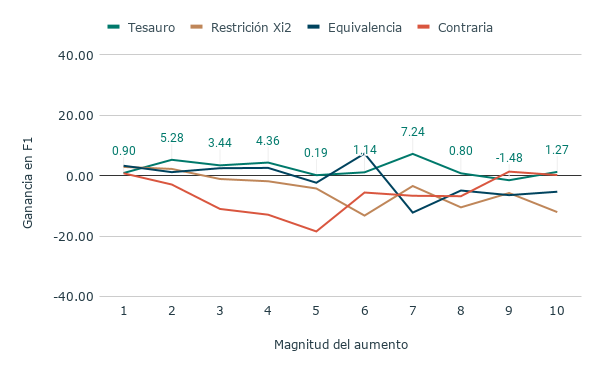
\includegraphics[width=\textwidth]{sections/figures/CNN2019.png}
        \caption{CNN}
    \end{subfigure}
    
  
    % \begin{subfigure}[b]{0.5\textwidth}
    %     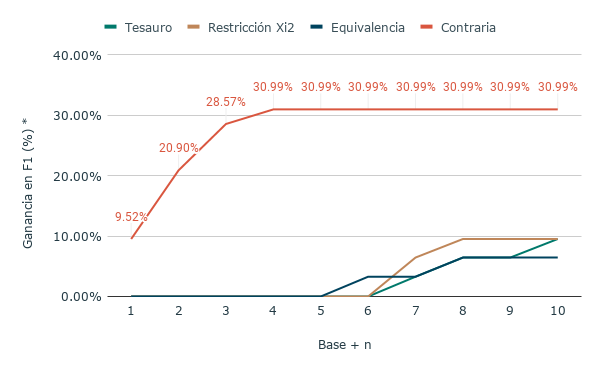
\includegraphics[width=\textwidth]{sections/figures/SVM2019.png}
    %     \caption{SVM}
    % \end{subfigure}
    % \hfill
    % \begin{subfigure}[b]{0.5\textwidth}
    %     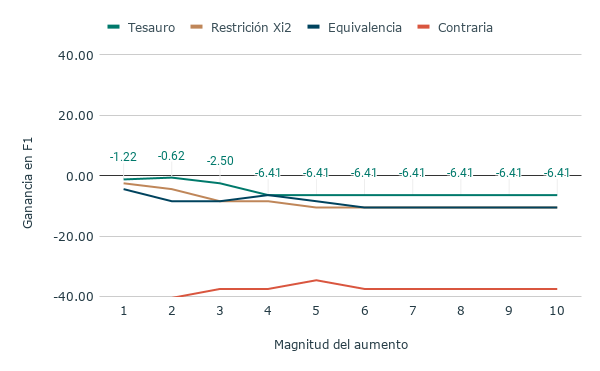
\includegraphics[width=\textwidth]{sections/figures/SVM-C2019.png}
    %     \caption{SVM-C}
    % \end{subfigure}

   
    \caption{Relación entre el aumento del conjunto de datos \textit{Depresión 2019} y la ganancia porcentual en F1.}
    \label{fig:aumento_n_depresion19}
\end{figure}
